\documentclass[11pt]{book}
\usepackage{graphicx,color,amssymb,amsmath,amsthm}
\usepackage{url}
\usepackage{fullpage}
\usepackage[ngerman]{babel}
\usepackage[toc,page]{appendix}
\usepackage[bw,framed]{includes/mcode}
% sets of numbers
\def\R{\mathbb{R}}
\def\C{\mathbb{C}}
\def\N{\mathbb{N}}
\def\Q{\mathbb{Q}}
\def\Z{\mathbb{Z}}
% caligraphic letters
\def\cA{\mathcal{A}}
\def\cC{\mathcal{C}}
\def\cI{\mathcal{I}}
\def\cJ{\mathcal{J}}
\def\cK{\mathcal{K}}
\def\cL{\mathcal{L}}
\def\cN{\mathcal{N}}
\def\cR{\mathcal{R}}
\def\cS{\mathcal{S}}
\def\cT{\mathcal{T}}
% greek letters
\def\a{\alpha}
\def\b{\beta}
\def\g{\gamma}
\def\d{\delta}
\def\k{\kappa}
\def\l{\lambda}
\def\s{\sigma}
% partial derivatives
\def\p{\partial}
% other greek letters
\def\veps{\varepsilon}
\def\vrho{\varrho}
\def\vphi{\varphi}
% weak convergence
\def\wto{\rightharpoonup}
% Matlab
\def\matlab{{\sc Matlab}}
% domains and boundaries
\def\O{\Omega}
\def\G{\Gamma}
% differential operators
\DeclareMathOperator{\diver}{div}
% environements
\newtheorem{definition}{Definition}
\newtheorem{lemma}[definition]{Lemma}
\newtheorem{satz}[definition]{Satz}
\newtheorem{theorem}[definition]{Theorem}
\newtheorem{korollar}[definition]{Korollar}
\newtheorem{bemerkung}[definition]{Bemerkung}
\newtheorem{beispiel}[definition]{Beispiel}
\newtheorem{algorithmus}[definition]{Algorithmus}
\parindent0mm
\begin{document}
%%% Einladen der Titelseite
\thispagestyle{empty}
\mbox{}
\begin{center}
\vspace*{2cm}
\hrule \vspace*{4mm}
{\huge \textsf{Fehlerkontrolle und adaptive Algorithmen}} \\[3mm]
\hrule \vspace*{3cm}
{\sc \huge Bachelorarbeit} \\[1cm]
vorgelegt von \\[.5cm]
{\Large Lukas Boschert} \\[1cm]
betreut von \\[.5cm]
{\Large Prof. Dr. S\"oren Bartels} \\[1.5cm]
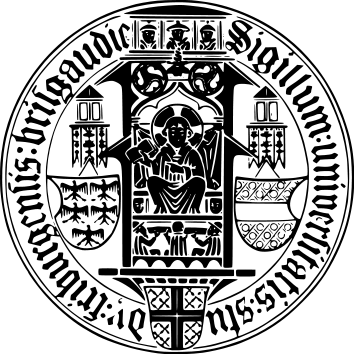
\includegraphics[width=4cm]{pics/alu-wappen}

\bigskip

{\sc Mathematisches Institut} \\
{\sc Fakult\"at f\"ur Mathematik und Physik} \\
{\sc Albert-Ludwigs-Universit\"at Freiburg} \\[1cm]
{\Large Freiburg, Juli 2017}

\end{center}
\mbox{}

\newpage
\thispagestyle{empty}
\mbox{}


%%%
\clearpage
\tableofcontents
\renewcommand{\thepage}{\roman{page}}
\setcounter{page}{1}
%%% Hier werden die Kapitel eingebunden
\chapter{Einleitung}
\renewcommand{\thepage}{\arabic{page}}
\setcounter{page}{1}
Um eine genauere Approximation einer Differentialgleichung zu erhalten, müssen wir die Gitterweite verringern. Doch mit mehr Gitterpunkten steigt auch der Rechenaufwand. Erfahrungsgemäß können wir feststellen, dass der Fehler zwischen Approximation und exakter Lösung an manchen Stellen größer ist als an anderen. Um die Rechenzeit effizient zu nutzen, wollen wir das Gitter nur an diesen Stellen verfeinern. Um dies möglich zu machen, brauchen wir berechenbare Indikatoren, die den Approximationsfehler kontrollieren. \\
Diese Arbeit stellt zunächst einen solchen Indikator für das Poisson-Problem $-\Delta u =f$ vor und liefert dann die nötigen Abschätzungen bezüglich des Fehlers. Im Anschluss wird der Algorithmus des adaptiven Gitters vorgestellt, der diesen Fehlerindikator nutzt, um das Approximationsgitter lokal bei großen Fehlerindikatoren zu verfeinern. Dabei muss sichergestellt werden, dass konforme Triangulierungen entstehen. \\
Als Abschluss werden die Ergebnisse auf ein Fallbeispiel angewendet und analysiert, inwiefern der entwickelte Algorithmus die Approximation verändert.
\chapter{Fehlerkontrolle}
Ziel des Kapitels ist es, einen berechenbaren, verlässlichen und effizienten Fehlerindikator zu finden. Die Erfahrung zeigt, dass die Größe des Winkels zwischen den zwei affinen Hyperflächen, welche von der Approximation auf den Elementen der Triangulation angenommen werden, ein guter Fehlerindikator sein könnte. Auf dieser Vermutung beruht die Definition des a posteriori (lat. erfahrungsbasiert; im Gegensatz zu a priori) Fehlerschätzers. 

\section{A Posteriori Fehlerschätzer}
Für die Definition des a posteriori  Fehlerschätzers wird eine Größe für die \verb|"|Schärfe\verb|"| der Kante benötigt. Dies liefert uns der Sprung. Je größer dieser, desto \verb|"|schärfer\verb|"| die Kante (Abbildung \ref{sprung}). 
\begin{definition}[Sprung]
	Sei $u_h\in\mathscr{S}^1(\mathscr{T}_h)$ und $S\in\mathscr{S}_h$ mit $S=T_1 \cap T_2$ für $T_1,T_2 \in \mathscr{T}_h$ verschieden, mit äußeren Normalen $n_{T_1,S},n_{T_2,S}$ auf S. Definiere den Sprung von $\nabla u_h$ über S als
	\[
	\llbracket \nabla u_h \cdot n_S\rrbracket = \nabla u_h|_{T_1} \cdot n_{T_1,S} + \nabla u_h|_{T_2} \cdot n_{T_2,S}
	\]
	Setze $\llbracket \nabla u_h \cdot n_S\rrbracket = 0$ für $S\subset \Gamma_D$
\end{definition} 

\begin{figure}[!htbp]
	\begin{center}
		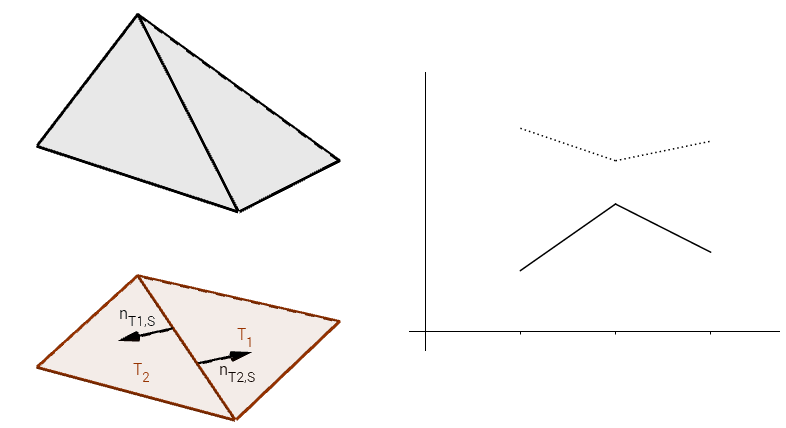
\includegraphics[width=12cm]{pics/Sprung.png}
	\end{center}
	\caption{\label{sprung}Zwei benachbarte Elemente mit darüberliegender Approximation (links). Schnitt entlang der Normalen mit großem (durchgezogene Linie) und kleinem (gestrichelte Linie) Sprung (rechts).}
\end{figure}

\begin{definition}[Verfeinerungsindikator]
	Für $u_h \in \mathscr{S}^1(\mathscr{T}_h) \text{ und } T \in \mathscr{T}_h$, definiere den Verfeinerungsindikator $\eta_T(u_h)$ durch
	\[
	\eta^2_T(u_h) = h^2_T\|f\|^2_{L^2(T)} + \sum_{S\in\mathscr{S}_h,S\subset\p T} h_S\|\llbracket \nabla u_h \cdot n_S\rrbracket\|^2_{L^2(S)} \]
\end{definition}
\begin{definition}[Fehlerschätzer]
	Für $u_h \in \mathscr{S}^1(\mathscr{T}_h) \text{ und } \mathscr{T}_h$ definiere den Fehlerschätzer $\eta_\mathscr{R}$ durch
	\[
	\eta_\mathscr{R}^2(u_h)=\sum_{T\in\mathscr{T}_h} \eta^2_T(u_h)
	\]
\end{definition}
Für $u$ Lösung des Poisson-Problems $-\Delta u = f$ soll nun gezeigt werden, dass gilt \\
\begin{center}
	\begin{tabular}{r c l l}
		$\|\nabla(u-u_h)\|$ & $\leq$ & $c_1 \eta_\mathscr{R}(u_h)$ &\textbf{Verlässlichkeit} \\
		$c_2 \eta_\mathscr{R}(u_h)$ &$\leq$& $\|\nabla(u-u_h)\|$ &\textbf{Effizienz} \\
	\end{tabular}
\end{center}
Der Fehlerindikator muss beide dieser Ungleichungen erfüllen. Der triviale Indikator $\eta(u_h)=1$ ist verlässlich aber nicht effizient, während $\eta(u_h)=0$ effizient aber nicht verlässlich ist. Beide sind für die Fehlerkontrolle und als Verfeinerungsindikator ungeeignet.
\section{Lokale Ungleichungen}
Um die Verlässlichkeit zu zeigen, wird ein Resultat über den Clément-Quasi-Interpolanten benötigt. Für dieses Resultat werden zunächst die lokale Poincaré- und die lokale Spur-Ungleichung vorgestellt.
\begin{definition}
	Sei $z \in \mathscr{N}_h$ Knoten. Definiere $\omega_z \subset \Omega$ als
	\[
	\omega_z = supp(\varphi_z)
	\]
	und $h_z = diam(\omega_z)$ Durchmesser von $\omega_z$
\end{definition}
\begin{bemerkung}
	Es gibt $c_{loc} > 0$, sodass für alle $T \in\mathscr{T}_h, z\in\mathscr{N}_h\cap T$ gilt
	\[
	h_z\leq c_{loc}h_T
	\]
\end{bemerkung}

\begin{lemma}[Lokale Poincaré-Ungleichung]\label{lemma}
	Sei $v \in H^1_D(\Omega)$ und $z\in \mathscr{N}_h.$ Sei $v_z= 0$ für $z\in \Gamma_D$ und sonst
	\[ v_z = |\omega_z|^{-1} \int_{\omega_z} v \quad dx
	\]
	Dann gibt es für alle $h > 0$ und $z \in \mathscr{N}_h$ eine Konstante $c_{p,z}>0$, sodass
	\[
	\|v-v_z\|_{L^2(\omega_z)}\leq c_{p,z}h_z\|\nabla v\|_{L^2(\omega_z)}.
	\]
\end{lemma}
\textbf{Beweis:}
\begin{itemize}
	\item[i)] 
	Für $z\in \mathscr{N}_h$ sei $\widehat{\omega}_z = h_z^{-1}(\omega_z - z)$. Dann ist nach Konstruktion $diam(\widehat{\omega}_z) = 1$ und
	\[
	\phi_z : \widehat{\omega}_z \rightarrow \omega_z, \quad \hat{x} \mapsto h_z\hat{x}+z
	\]
	affiner Diffeomorphismus mit $D\phi_z = h_zI$.
	
	\begin{figure}[!htbp]
		\begin{center}
			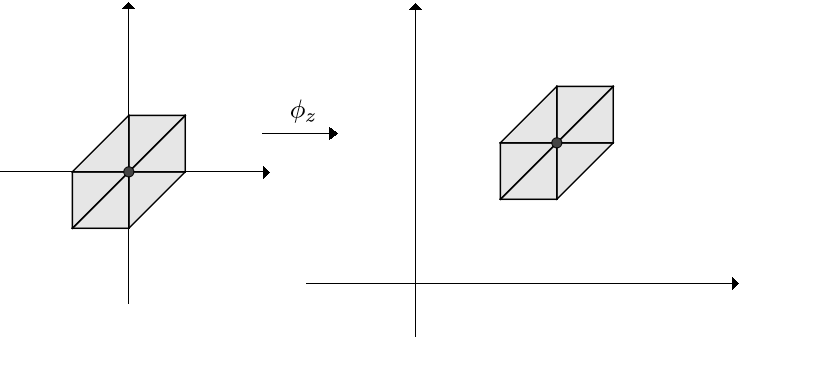
\includegraphics[width=15cm]{pics/omega.png}
		\end{center}
		\caption{Diffeomorphismus $\phi_z$ von $\widehat{\omega}_z$ nach $\omega_z$}
	\end{figure}

	\item[ii)] Mit der Standard Poincaré Ungleichung folgt für alle $\widehat{u}\in H^1(\widehat{\omega}_z)$
	\[
	\|\widehat{u}\|_{L^2(\widehat{\omega}_z)} \leq c_{p,z}\|\nabla \widehat{u}\|_{L^2(\widehat{\omega}_z)}
	\]
	wenn \[ \int_{\widehat{\omega}_z}\widehat{u}\:d\hat{x}=0 \text{ oder }\widehat{u}|_{\hat{\gamma}_z}
	\]
	für geschlossene Teilmenge ${\hat{\gamma}_z} \subset \p \widehat{\omega}_z$ mit positivem Flächenmaß.
	\item[iii)] Sei $v_z$ wie in Lemma \ref{lemma} definiert und $u= v-v_z\in H^1(\omega_z)$, dann erfüllt $\widehat{u} = u \circ \phi_z$ die Bedingungen für die Standard Poincaré-Ungleichung auf $\widehat{\omega}_z$.
	\item[iv)] Mit der Transformationsformel folgt:
	\begin{eqnarray*}
		\int_{\omega_z} u^2dx&=& \int_{\widehat{\omega}_z} \widehat{u}^2 | detD\phi_z|d\hat{x} \\
		&=& h_z^d\|\widehat{u}\|^2_{L^2(\widehat{\omega}_z)} \leq c^2_{p,z}h^d_z\|\nabla \widehat{u}\|^2_{L^2(\widehat{\omega}_z)} \\
		&=&c^2_{p,z}h^d_z\int_{\widehat{\omega}_z}| \nabla (u\circ\phi_z)|^2 d\hat{x} = c^2_{p,z}h^d_z \int_{\widehat{\omega}_z}|D\phi_z^\top(\nabla u)\circ\phi_z|^2 d\hat{x} \\
		&=& c^2_{p,z}h^d_zh^2_z\int_{\widehat{\omega}_z}|(\nabla u)\circ\phi_z|^2d\hat{x} 
		=c^2_{p,z}h^2_z\int_{\omega_z}|\nabla u|^2dx
	\end{eqnarray*} 
\end{itemize}
$\hfill \Box$

\begin{lemma}[Lokale Spur-Ungleichung]
	Sei $S \in  \mathcal{S}_h$ und $T_S \in \mathscr{T}_h$, sodass $S \subset \p T_s$. Dann
	gibt es die Konstante $c_{Tr} > 0$, sodass für alle $v\in H^1(\Omega)$ gilt:
	\[
	\|v\|^2_{L^2(S)} \leq c^2_{Tr}(h_S^{-1}\|v\|^2_{L^2(T_S)}+h_S\|\nabla v\|^2_{L^2(T_S)}).
	\]
\end{lemma}
\textbf{Beweis:}
Sei $\hat{S}$ die S entsprechende Seite auf dem Referenzelement $\hat{T}$. Auf dem Referenzdreieck gilt die Spur-Ungleichung
\[
\|\hat{v}\|^2_{L^2(\hat{S})} \leq c\|\hat{v}\|_{L^2(\hat{T})}\|\hat{v}\|_{H^1(\hat{T})}
\]
Nach der Transformation auf T
\[
\|v\|^2_{L^2(S)} \leq c\|v\|_{L^2(T)}(\|\nabla v\|_{L^2(T)}+h_S^{-1}\|v\|_{L^2(T)})
\]
Daraus folgt
\[
\|v\|^2_{L^2(S)} \leq c^2(h_S^{-1}\|v\|^2_{L^2(T)}+h_S\|v\|^2_{H^1(T)})
\]
$\hfill \Box$
\section{Clément-Quasi-Interpolant}
Im Gegensatz zum nodalen Interpolanten wird der Clément-Quasi-Interpolant über Mittelwerte definiert. Dies führt dazu, dass an Knoten nicht der exakte Wert angenommen wird. Dafür können auch nicht stetige Funktionen interpoliert werden.
\begin{definition}
    Sei $v \in L^1(\Omega) , z \in \mathscr{N}_h$
	\[
	v_z =  \left\{
	\begin{array}{ll}
		|\omega_z|^{-1} \int_{\omega_z} v dx& \text{f\"ur } z \in \mathscr{N}_h \setminus \Gamma_D\\
		0 &  \text{f\"ur } z \in \mathscr{N}_h \cap \Gamma_D
	\end{array}\right.
	\]
	Definiere den Clément-Quasi-Interpolant $\mathscr{J}_hv \in \mathscr{S}_D^1(\mathscr{T}_h)$ von v als
	\begin{displaymath}
		\mathscr{J}_hv = \sum_{z\in \mathscr{N}_h} v_z \varphi_z
	\end{displaymath}
\end{definition}
\begin{theorem}(Quasi-Interpolant-Abschätzung)
	Es existiert $c_\mathscr{J} > 0$, sodass f\"ur alle $v\in H^1_D(\Omega)$ gilt:
	\[
	\|\nabla\mathscr{J}_hv\| +\|h^{-1}_\mathscr{T}(v-\mathscr{J}_hv)\| +\|h^{-\frac{1}{2}}_\mathscr{S}(v-\mathscr{J}_hv)\|_{L^2(\cup\mathscr{S}_h)} \leq c_\mathscr{J}\|\nabla v\|
	\]
	mit $h_\mathscr{T}: \Omega \rightarrow  \R \text{ und } h_\mathscr{S}: \cup \mathscr{S}_h \rightarrow  \R$, definiert durch $h_\mathscr{T}|_T = h_T \text{ und }  h_\mathscr{S}|_S = h_S$ \\ f\"ur alle $T\in\mathscr{T}_h, S\in\mathscr{S}_h$.
\end{theorem}
\textbf{Beweis:}
\begin{itemize}
	\item[i)] Da für alle $x \in\Omega$ gilt $\sum_{\varphi\in\mathscr{N}_h}\varphi_z = 1$  ist $\sum_{z\in\mathscr{N}_h}\nabla \varphi_z=0$. Somit folgt mit Nulladdition
	\[
	\nabla \mathscr{J}_hv = \nabla \sum_{z\in \mathscr{N}_h}v_z\varphi_z = \sum_{z\in \mathscr{N}_h}(v_z-v) \nabla\varphi_z
	\]
	da $supp(\varphi_z)=\omega_z$
	\begin{eqnarray*}
		\| \nabla \mathscr{J}_hv\| &=& \int_{\Omega}(\sum_{z\in \mathscr{N}_h}(v_z-v) \nabla\varphi_z)\cdot \nabla \mathscr{J}_hvdx\\
		&\leq& \sum_{z\in \mathscr{N}_h}\int_{\omega_z}|v_z-v| |\nabla\varphi_z||\nabla \mathscr{J}_hv|dx
	\end{eqnarray*}
Die Inversenabschätzung liefert für alle z
\[
\|\nabla\varphi_z\|_{L^\infty(\omega_z)}\leq c_{inv}h^{-1}_z\|\varphi_z\|_{L^\infty(\omega_z)} =c_{inv}h^{-1}_z.
\]
Mit Hölder-, Cauchy-Schwarz- und der lokalen Poincaré-Ungleichung folgt
\begin{eqnarray*}
	\|\nabla\mathscr{J}_hv\|^2 &\leq&\sum_{z\in \mathscr{N}_h}\|v_z-v\|_{L^2(\omega_z)} \|\nabla\varphi_z\|_{L^\infty(\omega_z)}\|\nabla \mathscr{J}_hv\|_{L^2(\omega_z)}\\
	&\leq&c_{inv}c_p\sum_{z\in \mathscr{N}_h}\|\nabla v\|_{L^2(\omega_z)} \|\nabla \mathscr{J}_hv\|_{L^2(\omega_z)} \\
	&\leq&c_{inv}c_p\left(\sum_{z\in \mathscr{N}_h}\|\nabla v\|_{L^2(\omega_z)}^2\right)^{1/2} \left(\sum_{z\in \mathscr{N}_h} \|\nabla \mathscr{J}_hv\|_{L^2(\omega_z)}^2\right)^{1/2} \\
	&\leq&c_{inv}c_p(d+1)\|\nabla v\| \|\nabla \mathscr{J}_hv\|
\end{eqnarray*} 
In der letzten Abschätzung folgt aus endlicher Überlappung der $\omega_z$
\[
\sum_{z\in \mathscr{N}_h}\|\nabla v\|_{L^2(\omega_z)}^2 \leq (d+1)\sum_{T\in\mathscr{T}_h} \|\nabla v\|^2_{L^2(T)} = (d+1)\|\nabla v\|^2
\]
Teilen durch $\|\nabla\mathscr{J}_hv\|$ liefert die erste Abschätzung.
\item[ii)] Für beliebiges $\psi \in L^2(\Omega)$ gilt
\begin{eqnarray*}
	\int_{\Omega}\psi(v-\mathscr{J}_hv)dx &=& \int_{\Omega}\psi\left(v-\sum_{z\in \mathscr{N}_h}v_z\varphi_z\right)dx \\
	 &=& \int_{\Omega}\psi\left(\sum_{z\in \mathscr{N}_h}v\varphi_z-\sum_{z\in \mathscr{N}_h}v_z\varphi_z\right)dx\\
	 &=&\sum_{z\in \mathscr{N}_h}\int_{\omega_z} \psi (v-v_z)\varphi_zdx \\
	 &\leq&\sum_{z\in \mathscr{N}_h}\int_{\omega_z} |\psi| |v-v_z|dx \\
	 &\leq&c_p \sum_{z\in \mathscr{N}_h}\|\psi\|_{L^2(\omega_z)}h_z\|\nabla v\|_{L^2(\omega_z)}\\
	 &\leq&c_pc_{loc}\sum_{z\in \mathscr{N}_h}\|h_{\mathscr{T}}\psi\|_{L^2(\omega_z)}\|\nabla v\|_{L^2(\omega_z)}\\
	  &\leq&c_pc_{loc}(d+1)\|h_{\mathscr{T}}\psi\|\|\nabla v\|
\end{eqnarray*}
Durch geschicktes Wählen von $\psi = h_{\mathscr{T}}^{-2}(v-\mathscr{J}_hv)$ folgt die zweite Abschätzung.
\item[iii)]
Für alle $S\in\mathscr{S}_h$ definiere $T_S\in\mathscr{T}_h$, sodass $S\subset\p T_S$. Mit der lokalen Spur-Ungleichung, den Beweisschritten i) und ii) und da die Elemente sich maximal d+1 mal überlappen folgt
\begin{eqnarray*}
	\|h_{\mathscr{S}}^{1/2}(v-\mathscr{J}_hv)\|^2_{L^2(\cup \mathscr{S}_h)} &=& \sum_{S\in\mathscr{S}_h} h_S^{-1}\|v-\mathscr{J}_hv\|^2_{L^2(S)}\\
	 &=&c^2_{Tr} \sum_{S\in\mathscr{S}_h} (h_S^{-2}\|v-\mathscr{J}_hv\|^2_{L^2(T_S)} +
	 \|\nabla (v-\mathscr{J}_hv)\|^2_{L^2(T_S)})\\
	 &\leq&dc^2_{Tr} \sum_{T\in\mathscr{T}_h} (c_{loc}^2h_T^{-2}\|v-\mathscr{J}_hv\|^2_{L^2(T)} + \|\nabla (v-\mathscr{J}_hv)\|^2_{L^2(T)})\\
	 &=&dc^2_{Tr} (c_{loc}^2\|h_{\mathscr{T}}^{-2}(v-\mathscr{J}_hv)\|^2+ \|\nabla (v-\mathscr{J}_hv)\|^2)\\
	 &\leq&dc^2_{Tr}(c_{loc}^2c_1^2+c_2^2)\|\nabla v\|^2.
\end{eqnarray*}
Dies beweist die dritte Abschätzung.
$\hfill \Box$
\end{itemize}
\section{Verlässlichkeitsabschätzung}
Mit Hilfe des Quasi-Interpolanten lässt sich nun die erste Abschätzung zeigen, die für die Fehlerkontrolle notwendig ist.
\begin{theorem}[Verlässlichkeitsabschätzung]
	Sei $u\in H^1_0(\Omega)$ die schwache Lösung des Poisson-Problems \[-\Delta u = f ,\quad \Gamma_D = \p \Omega \text{ und } u|_{\p \Omega} = 0, \] und $u_h \in \mathscr{S}^1_0(\mathscr{T}_h)$ Galerkin-Approximation von u. Dann gibt es $c_R > 0$ , sodass
	\[\|\nabla(u-u_h)\|\leq c_R\eta_\mathscr{R}(u_h)
	\]
\end{theorem}
\textbf{Beweis:}
Sei $e = u-u_h$ der Approximationsfehler. Dann folgt aus der Galerkin-Orthogonalität und da u die schwache Lösung des Possoin-Problems ist
\begin{eqnarray*}
	\|\nabla e\|^2 &=& \int_{\Omega}\nabla e \cdot \nabla (e-\mathscr{J}_he)dx \\
	&=&\int_{\Omega} \nabla u \cdot \nabla (e-\mathscr{J}_he)dx -\int_{\Omega} \nabla u_h \cdot \nabla (e-\mathscr{J}_he)dx \\
	&=&\int_{\Omega} f (e-\mathscr{J}_he)dx -\int_{\Omega} \nabla u_h \cdot \nabla (e-\mathscr{J}_he)dx
\end{eqnarray*}
Da $\cup T = \Omega$,  $u|_T$ affin und somit $\Delta u|_T=0$ für alle $T\in\mathscr{T}_h$ ist , ergibt sich mit partieller Integration
\begin{eqnarray*}
	\int_{\Omega}\nabla u_h\cdot\nabla (e-\mathscr{J}_he) dx &=& \sum_{T\in\mathscr{T}_h} \int_{T} \nabla u_h \cdot \nabla (e-\mathscr{J}_he) dx \\
	&=& \sum_{T\in\mathscr{T}_h} \left(\int_{T} (-\Delta u_h) (e-\mathscr{J}_he) dx +\int_{\p T} (\nabla u_h \cdot n_T) (e-\mathscr{J}_he) ds\right) \\
	&=&\sum_{T\in\mathscr{T}_h} \int_{\p T} (\nabla u_h \cdot n_T) (e-\mathscr{J}_he) ds
\end{eqnarray*}
In der Summe wird über jede innere Seite zweimal integriert mit $u_h$ bezüglich der anliegenden Elemente und mit inversen Normalen. $(e-\mathscr{J}_he)$ ist bezüglich beider Elemente auf der Seite gleich. Da $(e-\mathscr{J}_he)|_{\p \Omega}=0$ und aus der Definition vom Sprung, folgt
\[
\sum_{T\in\mathscr{T}_h} \int_{\p T} (\nabla u_h \cdot n_T) (e-\mathscr{J}_he) ds =
\sum_{S\in\mathscr{S}_h} \int_{S} \llbracket \nabla u_h \cdot n_S\rrbracket (e-\mathscr{J}_he) ds
\]
Mit Hölder- und Schwarz-Ungleichungen folgt
\begin{eqnarray*}
	\|\nabla e\|^2 &=&  \sum_{T\in\mathscr{T}_h} \int_{T} f (e-\mathscr{J}_he)dx - \sum_{S\in\mathscr{S}_h} \int_{S} \llbracket \nabla u_h \cdot n_S\rrbracket (e-\mathscr{J}_he) ds \\
	&\leq&  \sum_{T\in\mathscr{T}_h}\|f\|_{L^2(T)} \|e-\mathscr{J}_he\|_{L^2(T)} + \sum_{S\in\mathscr{S}_h} \|\llbracket \nabla u_h \cdot n_S\rrbracket\|_{L^2(S)} \|e-\mathscr{J}_he\|_{L^2(S)}\\
	&\leq& \left( \sum_{T\in\mathscr{T}_h}h_T^2\|f\|_{L^2(T)}^2\right)^{1/2}\left( \sum_{T\in\mathscr{T}_h}h_T^{-2}\|e-\mathscr{J}_he\|_{L^2(T)}^2\right)^{1/2} \\
	&&+ \left(\sum_{S\in\mathscr{S}_h} h_S\|\llbracket \nabla u_h \cdot n_S\rrbracket\|_{L^2(S)}^2\right)^{1/2} \left(\sum_{S\in\mathscr{S}_h}h_S^{-1}\|e-\mathscr{J}_he\|_{L^2(S)}^2\right)^{1/2}\\
	&\leq& \left( \sum_{T\in\mathscr{T}_h}h_T^2\|f\|_{L^2(T)}^2\right)^{1/2}\|h_{\mathscr{T}_h}^{-1}e-\mathscr{J}_he\| \\
	&&+ \left(\sum_{S\in\mathscr{S}_h} h_S\|\llbracket \nabla u_h \cdot n_S\rrbracket\|_{L^2(S)}^2\right)^{1/2} \|h_{\mathscr{S}_h}^{-1/2}e-\mathscr{J}_he\|_{L^2(\Cup \mathscr{S}_h)}
\end{eqnarray*}
Mit der Quasi-Interpolanten-Abschätzung und der Ungleichung $a+b\leq \sqrt{2(a^2+b^2)}$ folgt

\begin{eqnarray*}
 \|\nabla e\| &\leq& c_{\mathscr{J}}\left( \sum_{T\in\mathscr{T}_h}h_T^2\|f\|_{L^2(T)}^2\right)^{1/2}
+ c_{\mathscr{J}}\left(\sum_{S\in\mathscr{S}_h} h_S\|\llbracket \nabla u_h \cdot n_S\rrbracket\|_{L^2(S)}^2\right)^{1/2} \\
 &\leq& \sqrt{2}c_{\mathscr{J}}\left( \sum_{T\in\mathscr{T}_h}h_T^2\|f\|_{L^2(T)}^2
 + \sum_{S\in\mathscr{S}_h} h_S\|\llbracket \nabla u_h \cdot n_S\rrbracket\|_{L^2(S)}^2\right)^{1/2}
\end{eqnarray*}
$\hfill \Box$
\section{Effizienz}
Für die Effizienzabschätzung werden zunächst Hilfsaussagen über die sogenannten Bubble-Funktionen bewiesen.
\begin{definition}
	Für $S \in \mathscr{S}_h$ Seite, definiere 
	\[
		\omega_S= int\left(\bigcup_{T\in\mathscr{T}_h,S\subset \p T}T\right)
    \]
    und für ein Element $T \in \mathscr{T}_h$ definiere
    \[
    \omega_T = \bigcup_{z\in\mathscr{N}_h,z\in T} \omega_z
    \]
\end{definition}
\begin{lemma}
	\leavevmode
	\begin{itemize}
		\item[1)]
		Für alle $T\in\mathscr{T}_h$ mit $T =conv\{z_1,z_2,...,z_{d+1}\}$ gibt es Konstanten $c_{e,1},c_{e,2}>0$,  sodass für die \textsf{Element Bubble-Funktion} $b_T = \varphi_{z_1}\varphi_{z_2}\cdots\varphi_{z_{d+1}} \in H^1(\Omega)\cap C(\overline{\Omega})$ gilt:
		\[
		supp(b_T)\subset T,\quad \int_{T} b_T =c_{e,1} |T|, \quad \|\nabla b_T\|_{L^2(T)} \leq c_{e,2}h_T^{d/2-1}
		\]
		\item[2)]
		Für alle $S\in\mathscr{S}_h$ mit $S =conv\{z_1,z_2,...,z_{d}\}$ gibt es Konstanten $c_{s,1},c_{s,2}>0$,  sodass für die \textsf{Seiten Bubble-Funktion} $b_S = \varphi_{z_1}\varphi_{z_2}\cdots\varphi_{z_{d}} \in H^1(\Omega)\cap C(\overline{\Omega})$ gilt:
		\[
		supp(b_S)\subset \omega_S,\quad \int_{S} b_S =c_{s,1} |S|, \quad \|\nabla b_S\|_{L^2(\omega_S)} \leq c_{s,2}h_S^{d/2-1}
		\]
	\end{itemize}
\end{lemma}
\textbf{Beweis:}
\begin{itemize}
	\item[i)] Damit $b_T\neq0$ müssen alle $\varphi_{z_{i}}\neq 0$. Somit folgt\[
	supp(b_T) = \cap_{i=1}^{d+1}supp(\varphi_{z_i})\subset T
	\]
	\item[ii)] Mit der Standard-Integralabschätzung folgt \[
	\int_{T}b_T \leq \max_{x\in T}b_T \int_{T}1 dx \leq |T|
	\]
	\item[iii)] Mit Standardabschätzung folgt \[
	\|b_T\| \leq \left(\int_{T}b_T^2dx\right)^{1/2} \leq \sqrt{|T|}\leq h_T^{d/2}
	\] Weiter gilt mit Transformation auf das Referenzelement $\hat{T}$
	\begin{eqnarray*}
		\|\nabla b_T\|^2 &=& \int_{\hat{T}} |\nabla b_{T}\circ \phi_z|^2 | detD\phi_z|d\hat{x} = h_T^dh^{-2}_T\int_{\hat{T}} |\nabla (b_T\circ \phi_z)|^2 d\hat{x} \\
		&=& h^{-2}_T h_T^d\| \nabla \widehat{b}_{\hat{T}}\|_{L^2(\hat{T})}^2 \leq c h^{-2}_T h_T^d \|\widehat{b}_{\hat{T}}\|_{L^2(\hat{T})}^2 \\
		&=& ch^{-2}_T\int_{\hat{T}} | (b_T\circ \phi_z)|^2 | detD\phi_z| d\hat{x}= ch^{-2}_T \| b_T\|^2
	\end{eqnarray*}
	Mit beiden Ungleichungen folgt die Behauptung.
\end{itemize}
Der Beweis für $b_S$ funktioniert analog.
$\hfill \Box$
\begin{figure}[!htbp]
	\begin{center}
		\includegraphics[width=16cm]{pics/bubble.png}
	\end{center}
	\caption{Bubble-Funktion $b_T$ auf einem Element(links). $b_S$ auf den an S anliegenden Elementen (rechts).}
\end{figure}
\newpage
Die Eigenschaften der Bubble-Funktionen nutzend, ist es nun möglich auch die zweite Ungleichung zur Fehlerkontrolle zu beweisen. 
\begin{theorem}[Lokale Effizienz]
	Sei $d=2, \Gamma_D = \p \Omega$ und $f\in L^2(\Omega)$ elementeweise konstant. Dann existiert eine Konstante $c_E > 0$, sodass für alle $T\in\mathscr{T}_h$ gilt
	\[
		c_E \eta_T^2(u_h)\leq \|\nabla (u-u_h)\|^2_{L^2(\omega_T)}
	\] 
\end{theorem}
\textbf{Beweis:}
\begin{itemize}
	\item[i)] 
	Für $T =conv\{z_1,z_2,...,z_{d+1}\} \in\mathscr{T}_h$ und $b_T = \varphi_{z_1}\varphi_{z_2}\cdots\varphi_{z_{d+1}}$, dann gilt mit partieller Integration und $\Delta u_h|_T = 0, b_T|_{\p T} = 0$
	\[
	\int_{\Omega} \nabla (u - u_h) \cdot \nabla b_T\:dx =\int_{\Omega} f b_T \:dx
	\]
    f ist konstant auf T mit Wert $f_T$ und Vorzeichen $\sigma_T$, dann gilt
    \[
    \sigma_T\int_{T}f_Tb_T\:dx=|f_T|\int_{T}b_T\:dx=c_{e,1}|f_T||T|= c_{e,1}|T|^{1/2}\|f_T\|_{L^2(T)}
    \]
    Mit $c_{loc}h_T \leq |T|^{1/2}$, Hölder-Ungleichung und $\|\nabla b_T\|_{L^2(T)} \leq c_{e,2}$ folgt
    \[
    h_T\|f\|_{L^2(T)}\leq \frac{c_{e,1}}{c_{loc}} |T|^{1/2}\|f\|_{L^2(T)} =\frac{\sigma_T}{c_{loc}}\int_{T}\nabla (u - u_h) \cdot \nabla b_T\:dx \leq c_{el} \|\nabla (u-u_h)\|_{L^2(T)}
    \]
    \item[ii)]
    Für $S =conv\{z_1,z_2,...,z_{d}\} = T_1 \cap T_2$ und $b_S = \varphi_{z_1}\varphi_{z_2}\cdots\varphi_{z_{d}}$ , dann gilt mit partieller Integration und $\Delta u_h|_{T_j} = 0, b_T|_{\p T_j\setminus S} = 0$
    \begin{eqnarray*}
    	\int_{\omega_S} \nabla (u-u_h)\cdot \nabla b_S \:dx &=& \int_{\omega_S} fb_S\:dx -\left(\int_{T_1} \nabla u_h\cdot \nabla b_S \:dx + \int_{T_2} \nabla u_h\cdot \nabla b_S \:dx\right) \\
    	&=& \int_{\omega_S} fb_S\:dx - \left(\int_{S} (\nabla u_h\cdot n_{T_1}) b_S \:ds + \int_{S} (\nabla u_h\cdot n_{T_2}) b_S \:ds\right)\\
    	&=& \int_{\omega_S} fb_S\:dx - \int_{S} \llbracket \nabla u_h \cdot n_S\rrbracket b_S\: ds
    \end{eqnarray*}
    $\llbracket \nabla u_h \cdot n_S\rrbracket$ ist konstant auf S. Sei $\sigma_S$ das Vorzeichen von $\llbracket \nabla u_h \cdot n_S\rrbracket$, dann gilt
    \[
    \sigma_S \int_{S} \llbracket \nabla u_h \cdot n_S\rrbracket b_S \:ds = c_{S,1}|\llbracket \nabla u_h \cdot n_S\rrbracket||S| =c_{S,1}\|\llbracket \nabla u_h \cdot n_S\rrbracket\|_{L^2(S)}|S|^{1/2}
    \] 
	Mit Hölder-Ungleichung, $\|\nabla b_S\|_{L^2(\omega_S)} \leq c_{S,2}$ und $\|b_S\|_{L^2(\omega_S)} \leq |\omega_S|^{1/2}$ gilt
	\begin{eqnarray*}
		c_{S,1}\|\llbracket \nabla u_h \cdot n_S\rrbracket\|_{L^2(S)}|S|^{1/2} &=& -\sigma_S\int_{\omega_S} \nabla (u-u_h)\cdot \nabla b_S\: dx +\sigma_S\int_{\omega_S} fb_S\:dx \\
		&\leq& c_{S,2} \|\nabla (u-u_h)\|_{L^2(\omega_S)} + |\omega_S|^{1/2}\|f\|_{L^2(\omega_S)}
	\end{eqnarray*}
	Mit $h_S =|S|$ und $|\omega_S|^{1/2} \leq c_{loc}h_S$ finden wir $c_{side}>0$, sodass	
	\[
	c_{side}^{-1}h_S^{1/2} \|\llbracket \nabla u_h \cdot n_S\rrbracket\|_{L^2(S)} \leq \|\nabla (u-u_h)\|_{L^2(\omega_S)} +h_S\|f\|_{L^2(\omega_S)}
	\]
	\item[iii)]
	Kombinieren von i), ii) und $a+b\leq \sqrt{2(a^2+b^2)}$ zeigt die Behauptung
	\begin{eqnarray*}
		\eta^2_T(u_h) &=& h^2_T\|f\|^2_{L^2(T)} + \sum_{S\in\mathscr{S}_h,S\subset\p T} h_S\|\llbracket \nabla u_h \cdot n_S\rrbracket\|^2_{L^2(S)} \\
		&\leq& c_{el}^2 \|\nabla (u-u_h)\|_{L^2(T)}^2 + \sum_{S\in\mathscr{S}_h,S\subset\p T}\|\nabla (u-u_h)\|_{L^2(\omega_S)}^2 +h_S^2\|f\|_{L^2(\omega_S)}^2\\
		&\leq&  c_E^{-2}\|\nabla (u-u_h)\|_{L^2(\omega_T)}^2
	\end{eqnarray*}
$\hfill \Box$
\end{itemize}
Da sich die $\omega_T$ nur endlich überlappen, folgt die Effizienzabschätzung
\[
\eta_\mathscr{R}(u_h) = \left( \sum_{T\in\mathscr{T}_h} \eta^2_T(u_h)\right)^{1/2} \leq \left( \sum_{T\in\mathscr{T}_h} c_E^{-2}\|\nabla (u-u_h)\|_{L^2(\omega_T)}^2\right)^{1/2} \leq c_E^{-1}(d+1)^{1/2} \|\nabla(u-u_h)\|
\]
\appendix
\chapter{Notation und Ungleichungen}
\begin{tabular}{l l}
	$\mathscr{T}_h$&Menge an Elementen die eine Triangulierung definieren\\
	$\mathscr{S}_h$&Menge von Seiten von Elementen einer Triangulierung\\
	& $\{S\subset\R^d|S= conv\{z_1,z_2,...,z_d\},z_1,z_2,...,z_{d+1}\in\mathscr{N}_h, T\in\mathscr{T}_h, T= conv\{z_1,z_2,...,z_{d+1}\}\}$\\
	$\mathscr{N}_h$&Menge von Knotenpunkten\\
	$h_T,h_S,h_Z$&lokale Gitterweiten\\
	$\varphi_z$&Nodale Basisfunktion von Knoten z\\
	$\Gamma_D$&Dirichlet Rand\\
	$\mathscr{S}^1(\mathscr{T}_h)$&Stetige auf Elementen von $\mathscr{T}_h$ affine\\
	$\mathscr{S}^1_D(\mathscr{T}_h)$&Funktionen aus $\mathscr{S}^1(\mathscr{T}_h)$ die auf $\Gamma_D$ verschwinden\\
	$H^1(\Omega)$ &Hilbertraum $W^{1,2}(\Omega)$\\
\end{tabular}
\\  \\ \\ \\
\textbf{Cauchy-Schwarz Ungleichung}
Für alle $x,y\in\R^n$ gilt
\[
x\cdot y =\sum_{i=1}^{n} x_iy_i\leq\left(\sum_{i=1}^{n}x_i^2\right)^{1/2}\left(\sum_{i=1}^{n}y_i^2\right)^{1/2} =|x||y|
\]\\
\textbf{Hölder Ungleichung}
Für $f\in L^p(\Omega)$ und $g\in L^q(\Omega)$ und $1\leq p, q\leq \infty$ mit $\frac{1}{p}+\frac{1}{q}=1$. Dann gilt
\[
\int_{\Omega} fg\:dx\leq \|f\|_{L^p(\Omega)} \|g\|_{L^q(\Omega)}
\]\\
\textbf{Poincaré Ungleichung}
Für $v\in W^{1,p}(\Omega)$ mit $1\leq p \leq \infty$ und $v|_{\Gamma_D}=0$ oder $\int_{\Omega}v\:dx =0$. Dann gibt es $c_P>0$, sodass
\[
\|v\|_{L^p(\Omega)} \leq c_P\|\nabla v\|_{L^p(\Omega)}
\]\\

\textbf{Spur Ungleichung}
Für $v\in W^{1,p}(\Omega)$ mit $1\leq p \leq \infty$ . Dann gibt es $c_{Tr}>0$, sodass
\[
\|v\|_{L^p(\p \Omega)} \leq c_{Tr}\|v\|_{W^{1,p}(\Omega)}
\]
%%%
\bibliography{literature}
\addcontentsline{toc}{chapter}{Literaturverzeichnis} 
\bibliographystyle{amsalpha}
\chapter*{Zusammenfassung}
\addcontentsline{toc}{chapter}{Zusammenfassung} 

Mithilfe des erfahrungsbasierten, berechenbaren Fehlerindikators
\[
\eta_\mathscr{R}(u_h)=\left(\sum_{T\in\mathscr{T}_h} \eta^2_T(u_h)\right)^{1/2}
\]
mit
$
\eta^2_T(u_h) = h^2_T\|f\|^2_{L^2(T)} + \sum_{S\subset\p T} h_S\|\llbracket \nabla u_h \cdot n_S\rrbracket\|^2_{L^2(S)} 
$, ist es möglich den Fehler einer Approximation des Poisson Problems zu kontrollieren, also den Fehler nach oben und unten zu beschränken. So kann die Approximation, insbesondere lokal, ohne Kenntnis der exakten Funktion bezüglich der Exaktheit beurteilt werden. Es ist bekannt, dass mit der Gitterweite der Fehler sinkt. So folgt für jedes Element $T \in \mathscr{T}_k$ und Elemente $T_i'\in \mathscr{T}_{k+1}$ mit $\overset{.}{\cup} T_i' =T$, da $\eta_T$ den Fehler nach oben beschränkt, dass $\eta_T\geq \sum \eta_{T'_i}$ Somit wird $\eta_\mathscr{R}$ kleiner, wenn einzelne $T$ verfeinert werden. Da $\eta_\mathscr{R}$ den Fehler nach oben beschränkt, reicht es also $\eta_\mathscr{R}$ zu minimieren, um den Fehler zu minimieren. \\
Aus dieser Erkenntnis folgt der Algorithmus des adaptiven Gitters. Dieser Algorithmus schafft es ohne weitere Kenntnisse über die exakte Funktion ein Gitter zu entwickeln, das an Problemstellen wie zum Beispiel Singularitäten stark verfeinert ist. Mit dieser Adaptivität folgt jedoch auch potenziell mehr Rechenaufwand, da nicht einmal, sondern mehrfach Approximiert wird. bis auf die letzte werden alle Approximationen wieder verworfen. Sie dienten nur dafür die Fehlerindikatoren zu berechnen.\\
Das adaptive Gitter hat im Vergleich zu einem Gitter mit gleichmäßiger Gitterweite, auf denen eine Approximation vergleichbare Fehler liefert, sehr viel weniger Knoten. Da das Approximieren auf einem Gitter mit n-Knoten in $\mathcal{O}(n^2)$ liegt, kann nicht a priori gesagt werden ob das adaptive Gitter Verfahren schneller ist. Dies hängt von der Differenzialgleichung, dem Gebiet und auch von der Wahl des Parameters Theta ab, der entscheidet wie viele der Elemente in der Triangulierung verfeinert werden. Wird Theta klein gewählt, dann werden viele Elemente verfeinert. Der Algorithmus konvergiert in weniger Schritten als für größere Theta. Jedoch enthält die Triangulierung, die für die selbe Fehlerschwelle entsteht, für größeres Theta weniger Knoten. Soll also eine Approximation einmalig berechnet und gespeichert werden, sollte ein möglichst großes Theta gewählt werden, um Apeicherplatz zu sparen. \\
Mit mehr Wissen über die exakte Lösung ist es auch möglich, ein spezielles Gitter für die Approximation zu entwickeln. Zum Beispiel kann gezeigt werden, dass das die Lösung des Poisson Problems an einspringenden Ecke Singularitäten besitzt. So ist es möglich, an den bekannten Problemstellen lokal zu verfeinern. Wie bei einem Gitter mit gleichmäßiger Gitterweite wird hier nur einmal Approximiert. Wie in der Argumentation oben ist kein Verfahren a priori schneller. Im Nachteil zum adaptiven Gitter kann es hier aber sein, dass der Fehler an den nicht speziell verfeinerten Stellen, den Fehler an den Problemstellen durch Überverfeinerung an diesem und sehr große Gitterweite sonst, überwiegt. Außerdem werden Problemstellen, die vorher nicht bekannt sind, nicht speziell behandelt. \\
Im Allgemeinen gilt, wenn die $\eta_{T}$ für die Approximierung auf dem Anfangsgitter ungefähr gleich für alle T sind, also es keine Stellen gibt, an denen der Fehler besonders groß ist, dass das adaptive Gitterverfahren nicht besonders Rechen effizient ist. Im Gegensatz dazu ist das Verfahren besonders effektiv, wenn die Unterschiede zwischen kleinstem und größtem $\eta_{T}$ besonders groß sind. Dies kann Beispielsweise passieren, wenn die exakte Lösung ein Plateau hat. Im Fall der Phasenfeldgleichung, die die Vermischung zweier Substanzen beschreibt, ist das Verfahren mit auf die Gleichung angepassten $\eta_{T}$, sodass die Effizienz- und Verlässlichkeitsabschätzung erfüllt sind, zum Beispiel sehr effektiv, da am Phasenübergang sehr viele, und in den Phasen nur sehr wenige Knoten benötigt werden, um eine gute Approximierung zu erhalten.
\chapter*{Erkl\"arung}
\addcontentsline{toc}{chapter}{Erkl\"arung} 

Hiermit erkl\"are ich, dass ich die vorliegende Bachelorarbeit 
selbstst\"andig verfasst und keine anderen als die angegebenen
Quellen und Hilfsmittel verwendet habe. 

\bigskip
\bigskip

\noindent
Freiburg, ??XX. Februar 2014?? \hfill \underline{\hspace{5cm}} \hspace*{.5cm} \\
\mbox{ } \hfill Lukas Boschert \hspace*{2cm}
%%% Kompilieren
% pdflatex main.tex; bibtex main; pdflatex main.tex
\end{document}